\section{Specific UI Research}
\label{research:SpecificUIResearch}
To understand the workflows of various competitors platforms I created new accounts and went through the process of storing a few notes to understand how each platform functions
\subsection*{Obsidian:}
\begin{figure}[h]
    \centering
    \begin{minipage}[H]{0.32\textwidth}
        \centering
        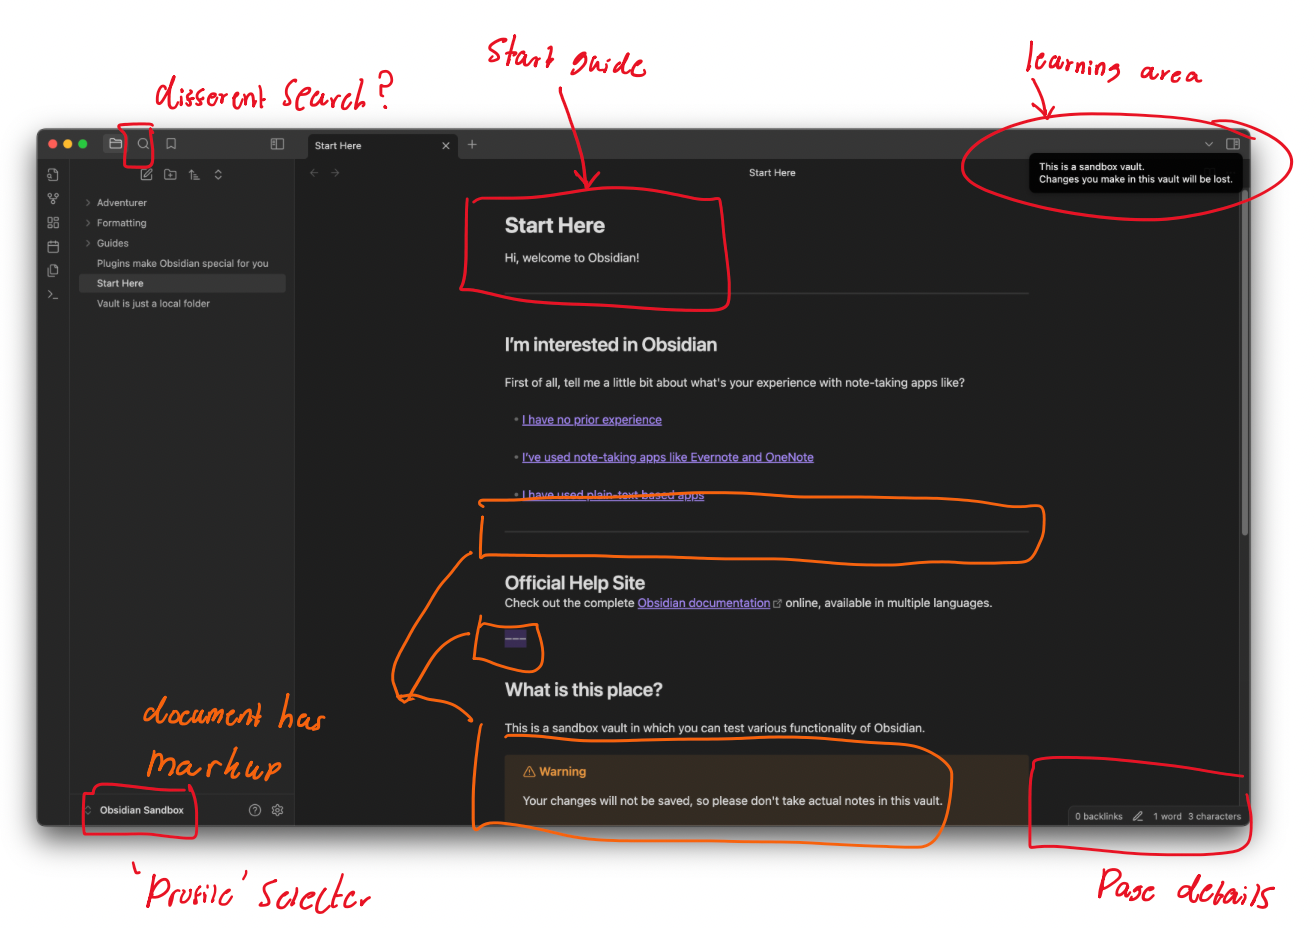
\includegraphics[width=\textwidth]{Research/15_SpecificUIResearch/media/obsidian1.png}
        \caption*{Obsidian Screenshot 1}
    \end{minipage}
    \hfill
    \begin{minipage}[H]{0.32\textwidth}
        \centering
        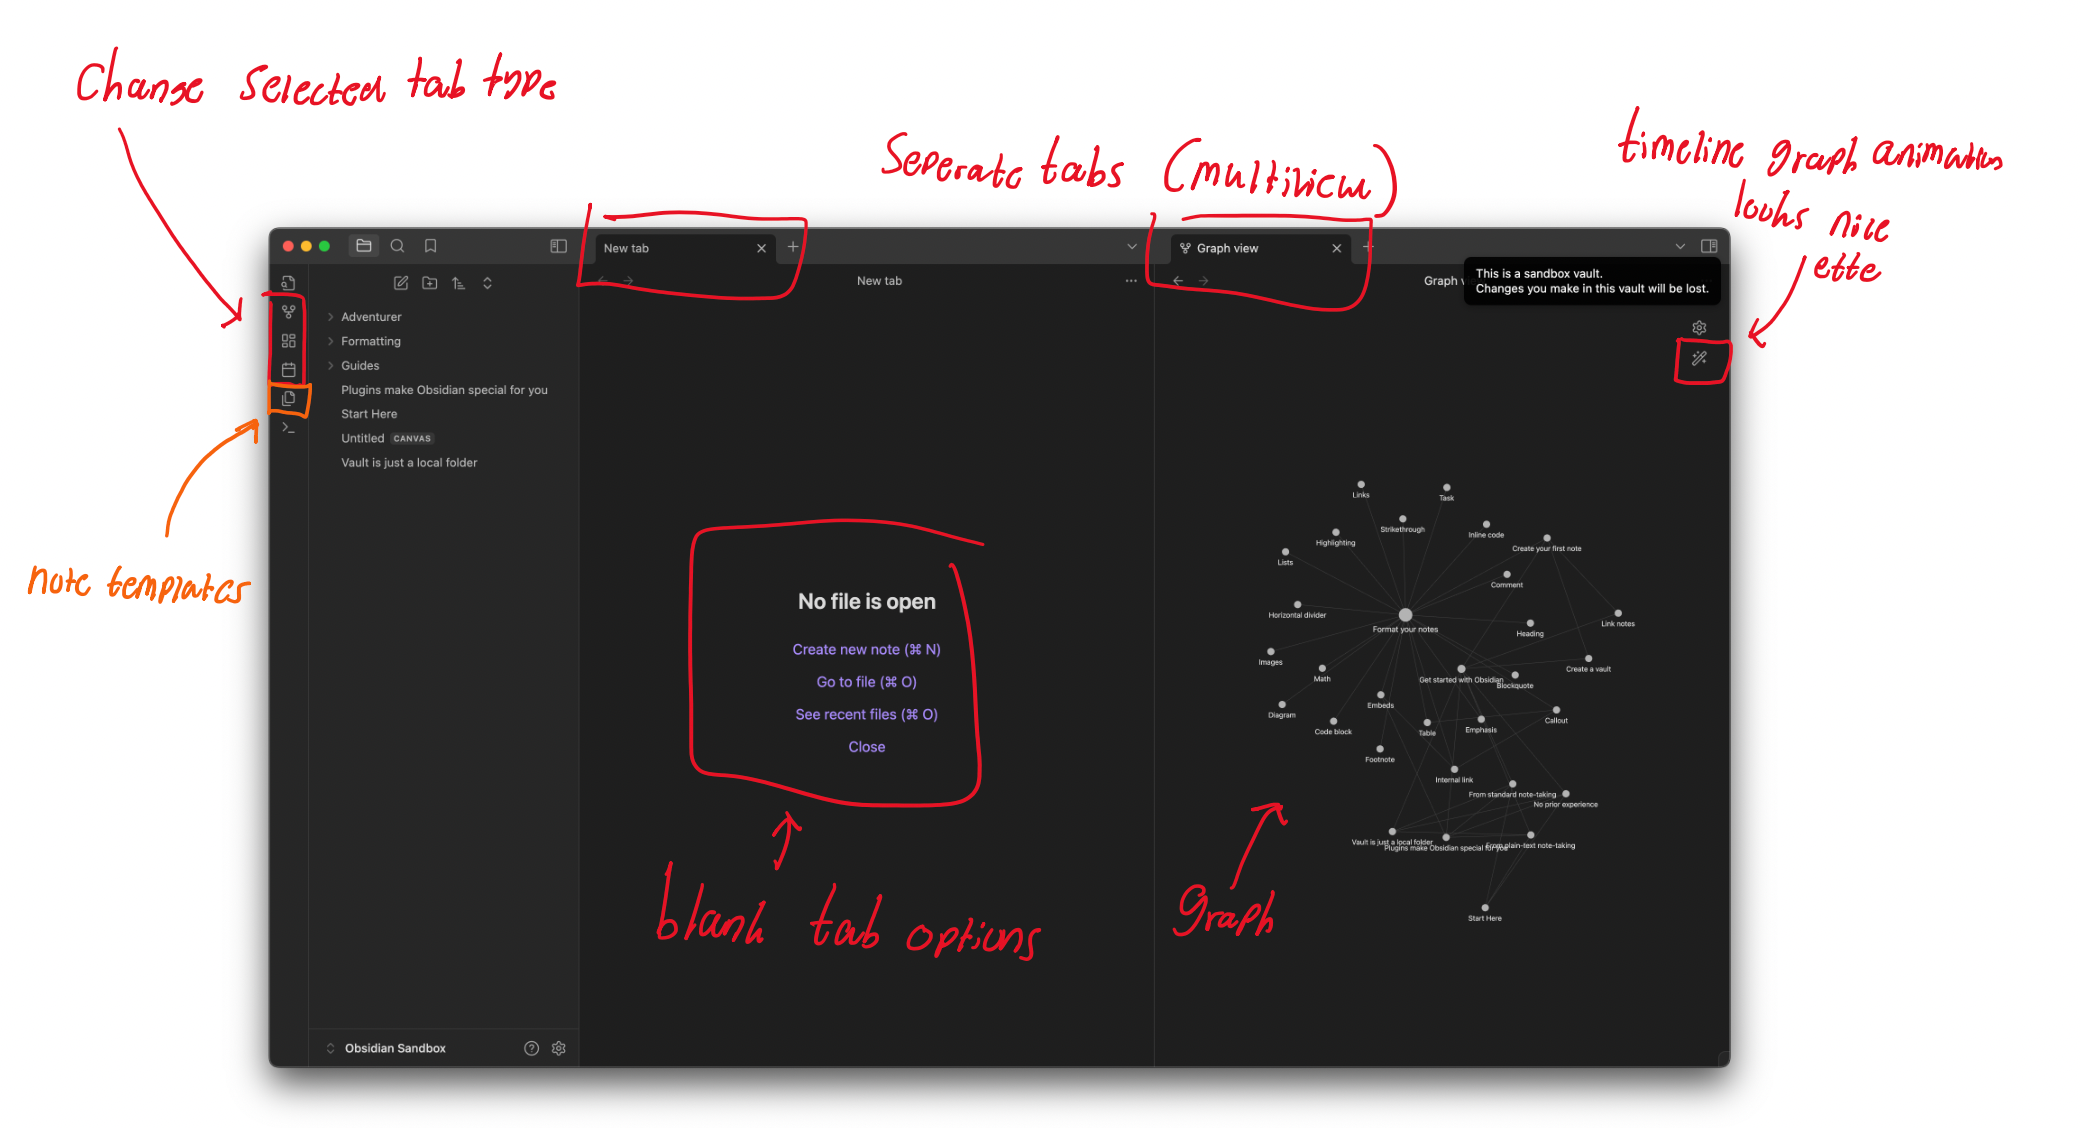
\includegraphics[width=\textwidth]{Research/15_SpecificUIResearch/media/obsidian2.png}
        \caption*{Obsidian Screenshot 2}
    \end{minipage}
    \hfill
    \begin{minipage}[H]{0.32\textwidth}
        \centering
        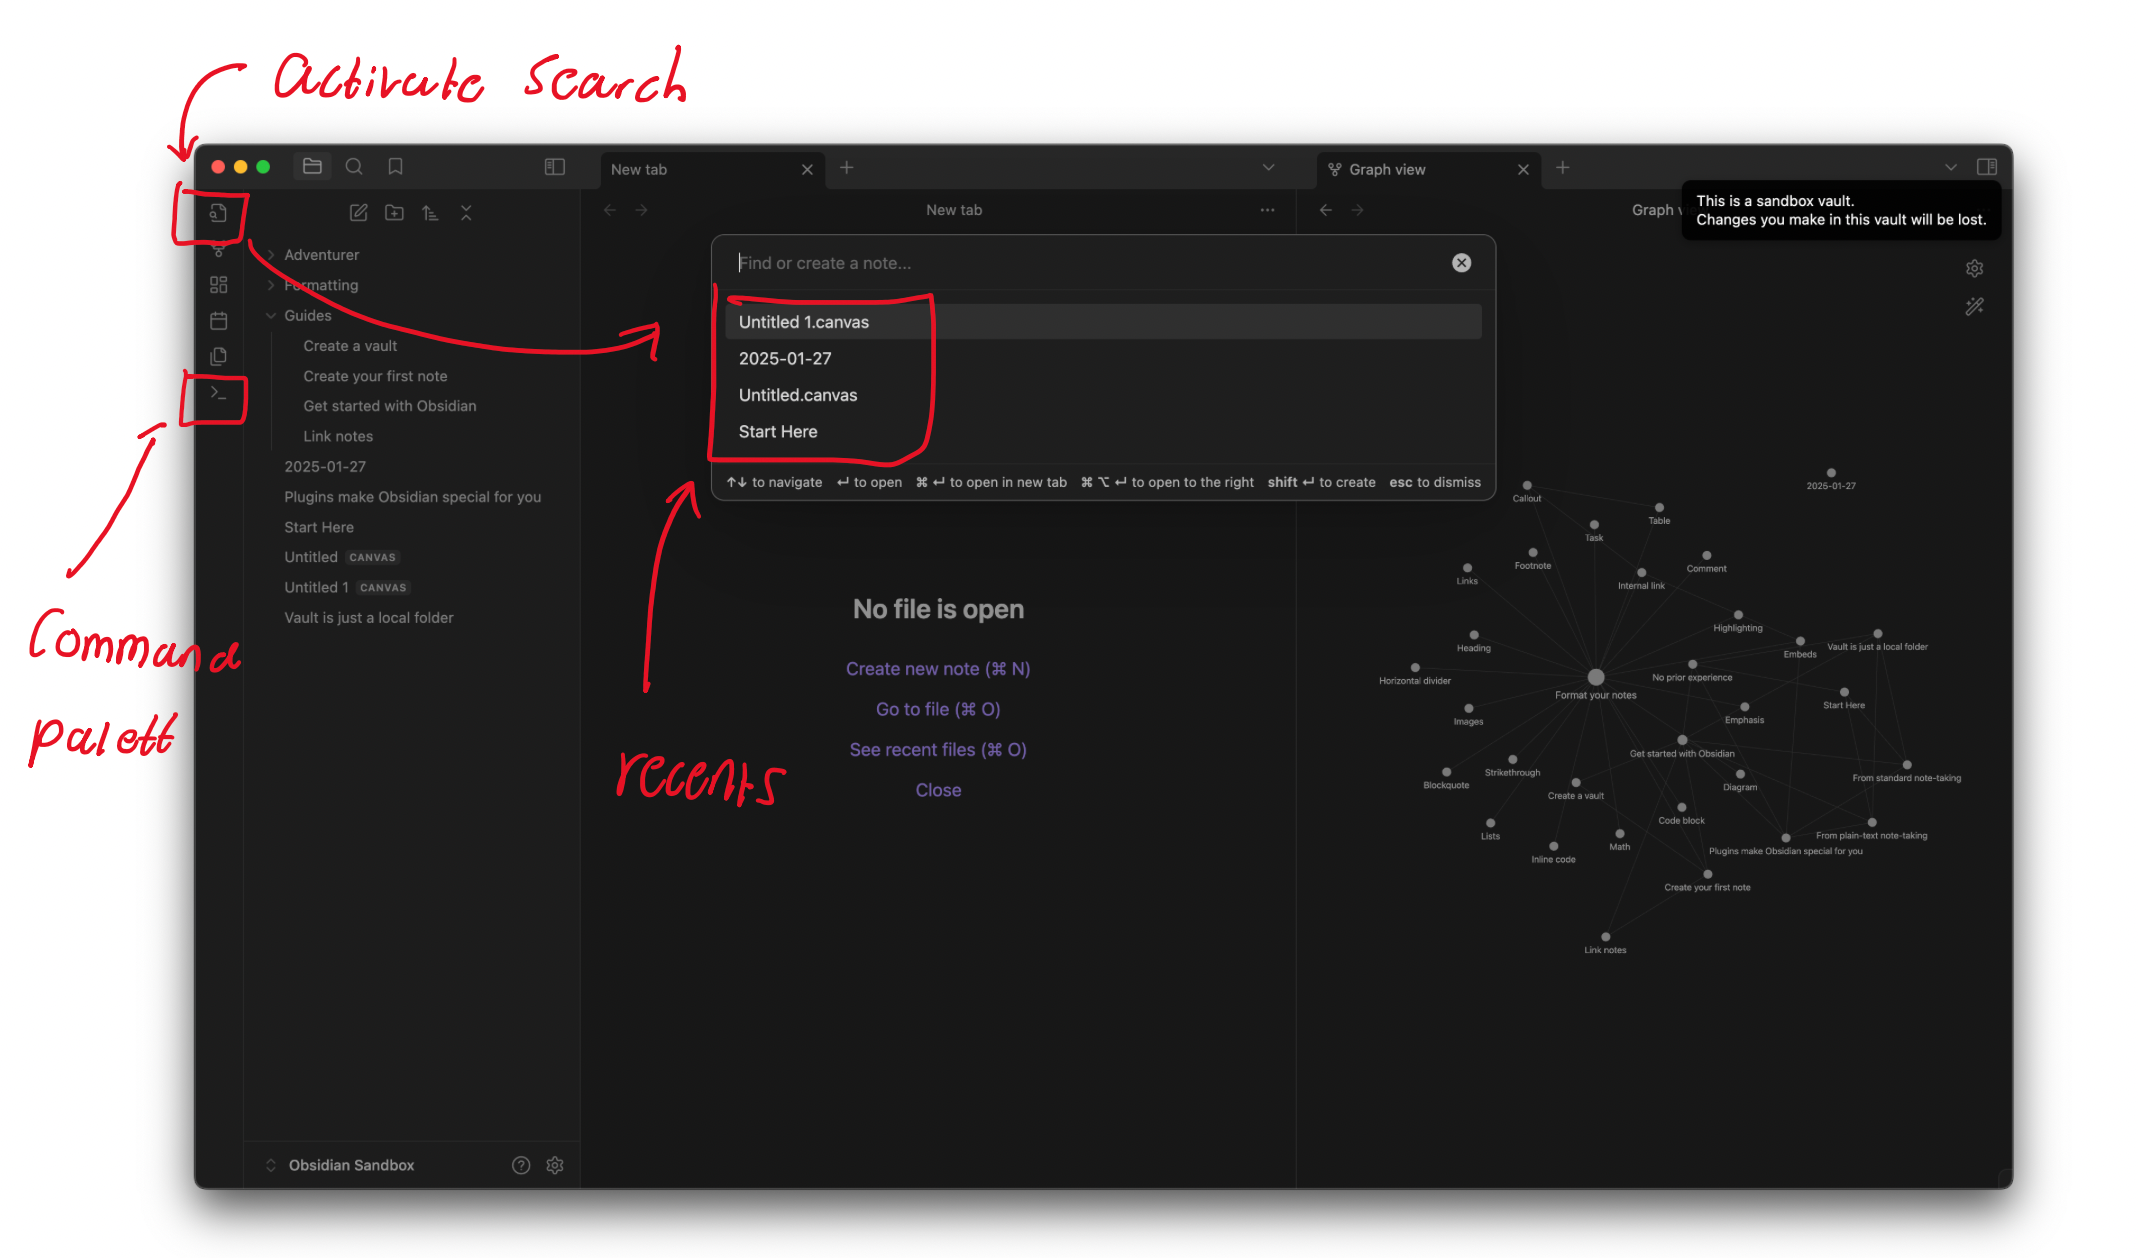
\includegraphics[width=\textwidth]{Research/15_SpecificUIResearch/media/obsidian3.png}
        \caption*{Obsidian Screenshot 3}
    \end{minipage}
    \caption{Obsidian UI Screenshots}
\end{figure}

As a 'first time user' to obsidian I was greeted by this first screenshot showing me a couple of the software's features however I couldn’t easily find a tutorial in the software which seemed un-intuitive. In fact this does carry throughout many design decisions I came across during my time using the software. Whilst I am sure each icon is quick to press and keyboard shortcut intuitive once you have mastered the platform at the moment is seems very alien to me. Simple functions like changing the type of a tab requires clicking to the far left of the interface and the search tool is positioned as a small icon stuck to the far left. Despite this there are a number of ideas I really like and I can learn from. The graph of nodes is already a huge inspiration and has been mentioned many times. The easy access to a library of stock and custom note templates (useful for methods such as Cornell notes I imagine) is powerful, the easily visible and all encompassing search menu (whilst hard to initially open) is easy to use and the use of tabs throughout the interface make it flexible to tailor to my exact working requirements such as seeing multiple notes side by side or quickly switching notes - I definitely want to implement this system in my webapp

Takeaways:
\begin{itemize}
	\item Flexible panels which can each change view type give amazing flexibility and customisability to user
	\item Graph view animation is smooth
	\item Central and focused search bar searches everything in application
	\item Easily accessible templates
	\item User never sees a blank screen - always well labelled options front and centre
\end{itemize}

\subsection*{OneNote:}
\begin{figure}[H]
    \centering
    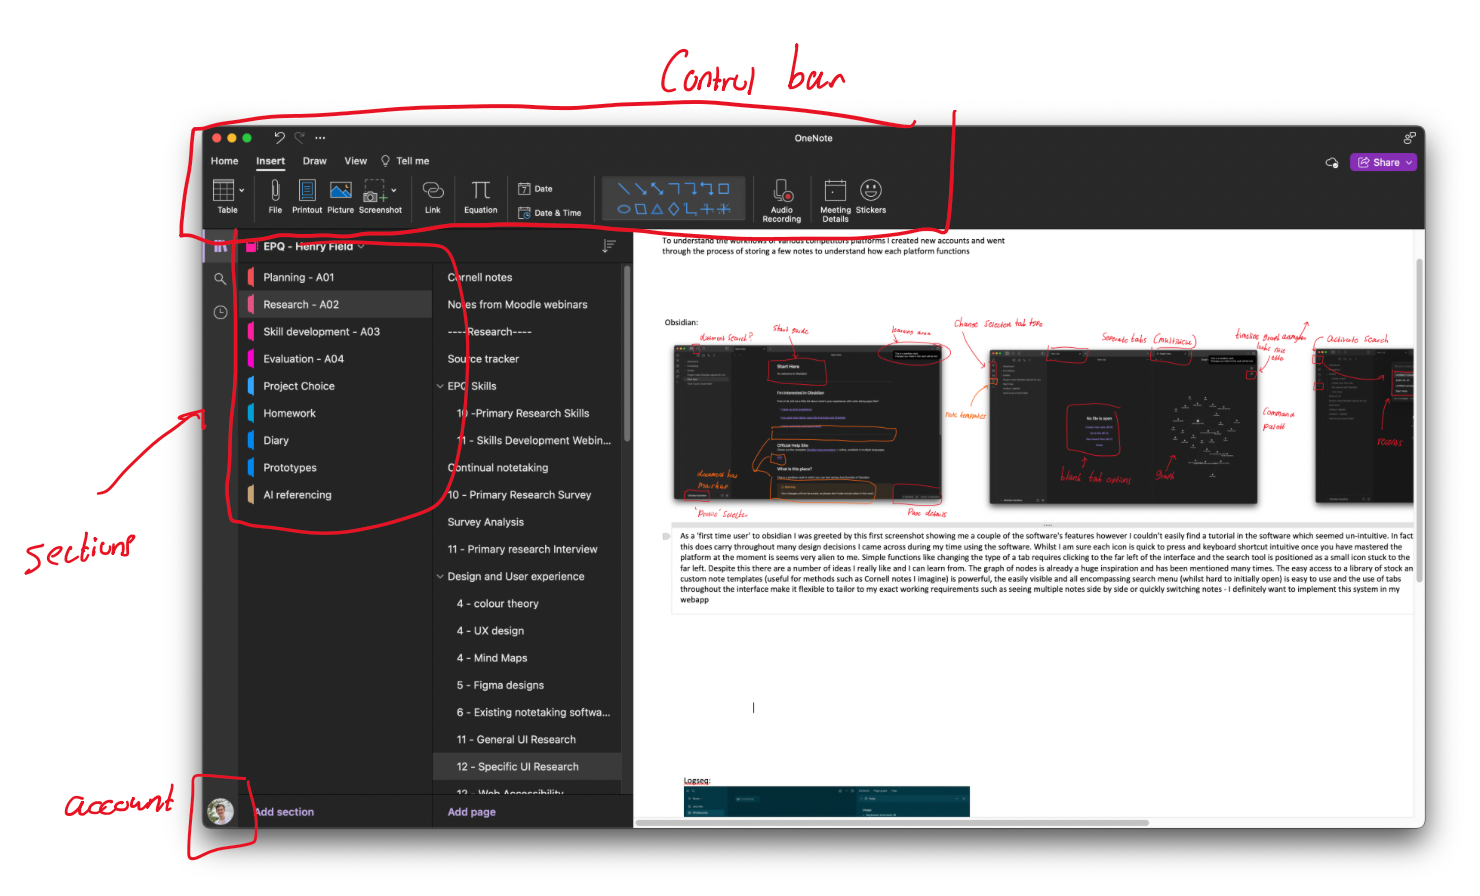
\includegraphics[width=0.5\textwidth]{Research/15_SpecificUIResearch/media/onenote1.png}
    \caption{OneNote UI Screenshot}
\end{figure}

Being my most used notes app, I have become very used to OneNote with all of its ups and downs. The UI styling follows Microsoft's global design language containing a group of top bar tabs which give you control over your content, sidebar which shows you all of your notes and right hand side (expandable) section with the actual note content. While there are few issues with it I (and many other from my survey) find it lacking features and frustrating to use when trying to multitask due to a lack of modular  panels the interface is reliable and I rarely find myself lost in a menu / missing a button
Takeaways:
\begin{itemize}
    \item Easy and intuitive to find controls
    \item Visible Controls all work no matter which viewing mode is active
    \item Can hide sidebars to focus on content
\end{itemize}

\subsection*{Notion:}
\begin{figure}[H]
    \centering
    \begin{minipage}[b]{0.48\textwidth}
        \centering
        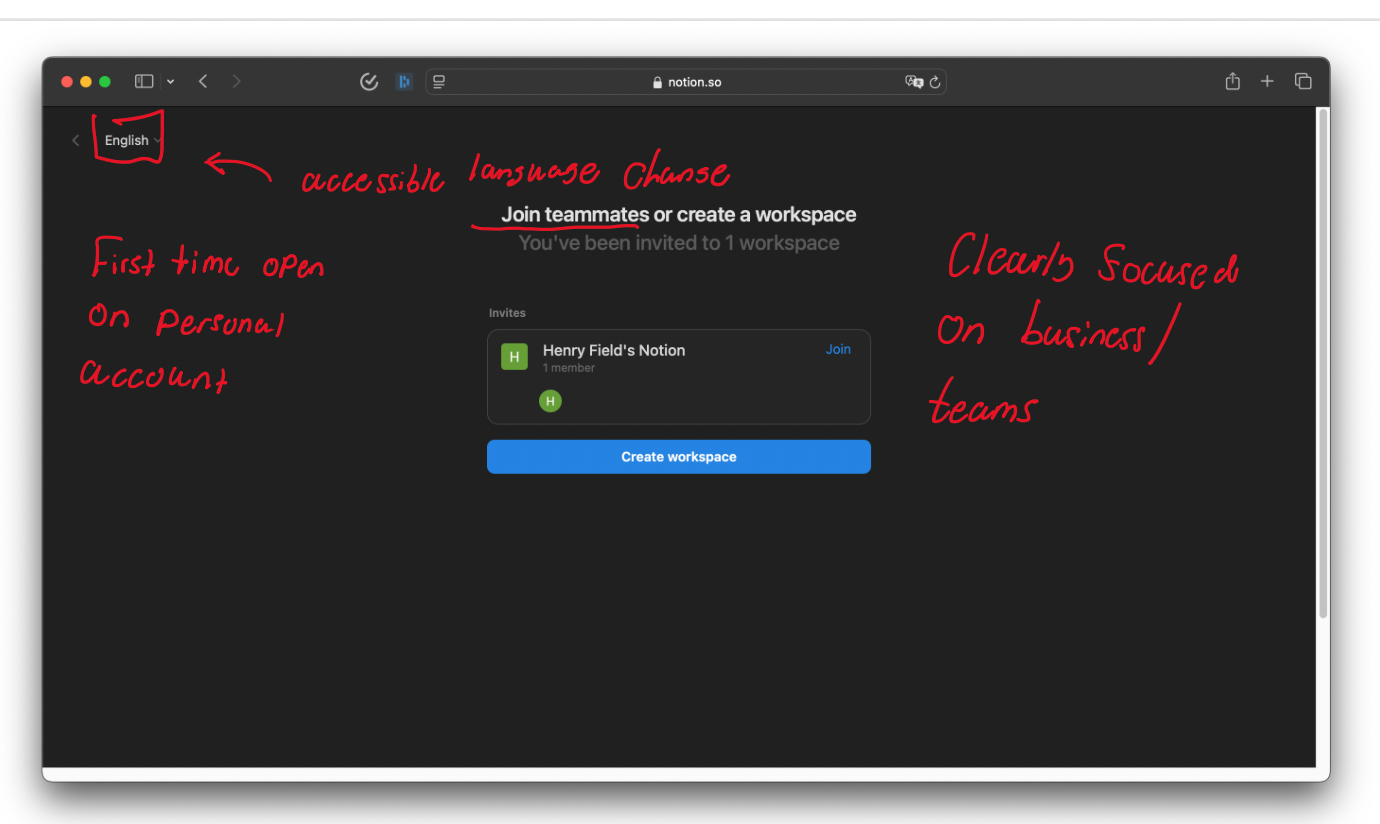
\includegraphics[width=\textwidth]{Research/15_SpecificUIResearch/media/notion1.png}
        \caption*{Notion Screenshot 1}
    \end{minipage}
    \hfill
    \begin{minipage}[b]{0.48\textwidth}
        \centering
        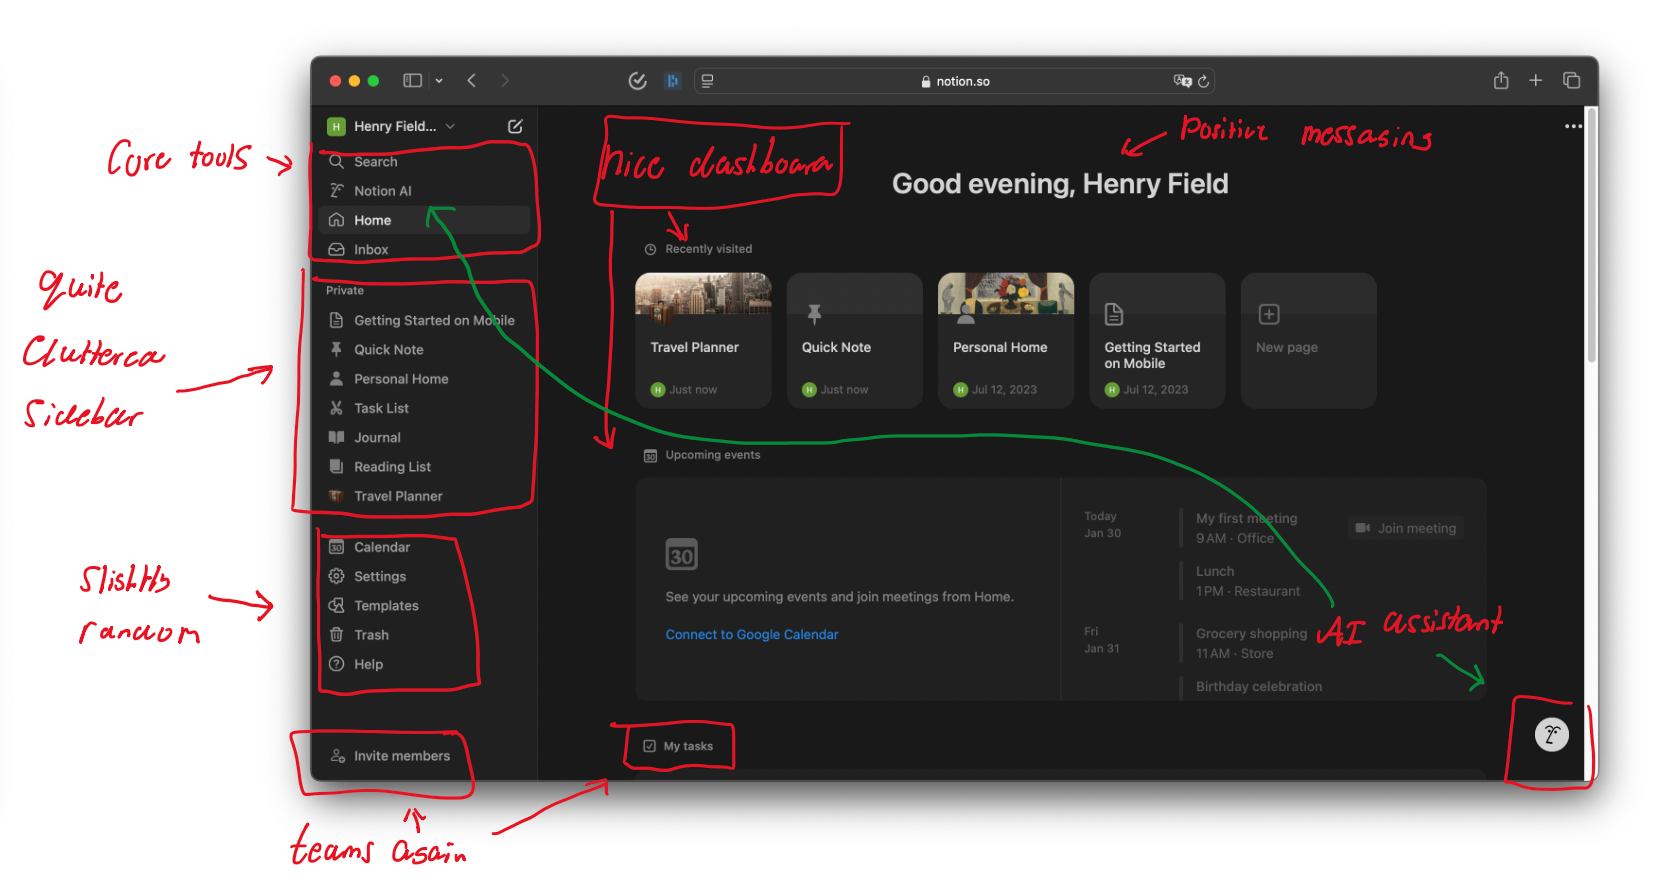
\includegraphics[width=\textwidth]{Research/15_SpecificUIResearch/media/notion2.png}
        \caption*{Notion Screenshot 2}
    \end{minipage}
    \vspace{0.5em}
    \begin{minipage}[b]{0.48\textwidth}
        \centering
        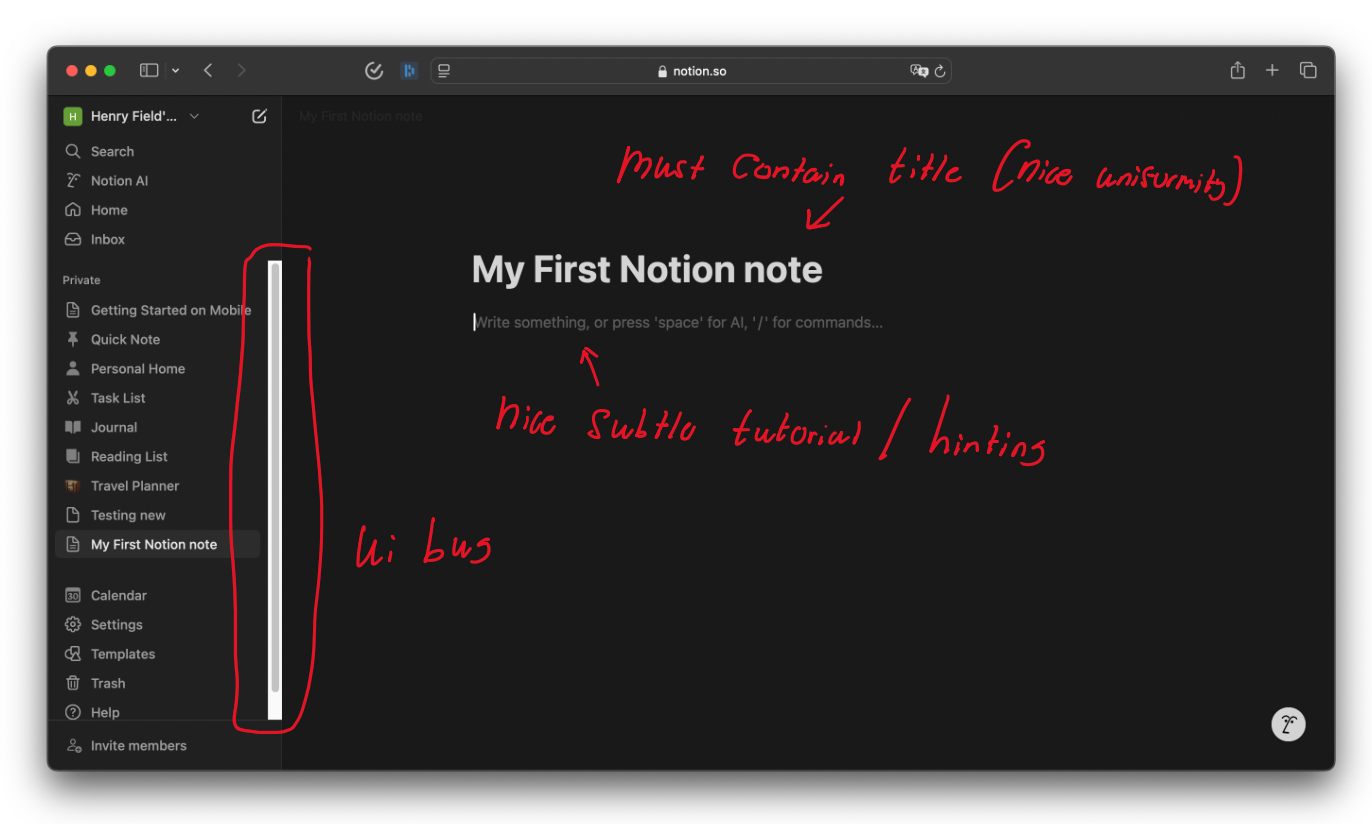
\includegraphics[width=\textwidth]{Research/15_SpecificUIResearch/media/notion3.png}
        \caption*{Notion Screenshot 3}
    \end{minipage}
    \hfill
    \begin{minipage}[b]{0.48\textwidth}
        \centering
        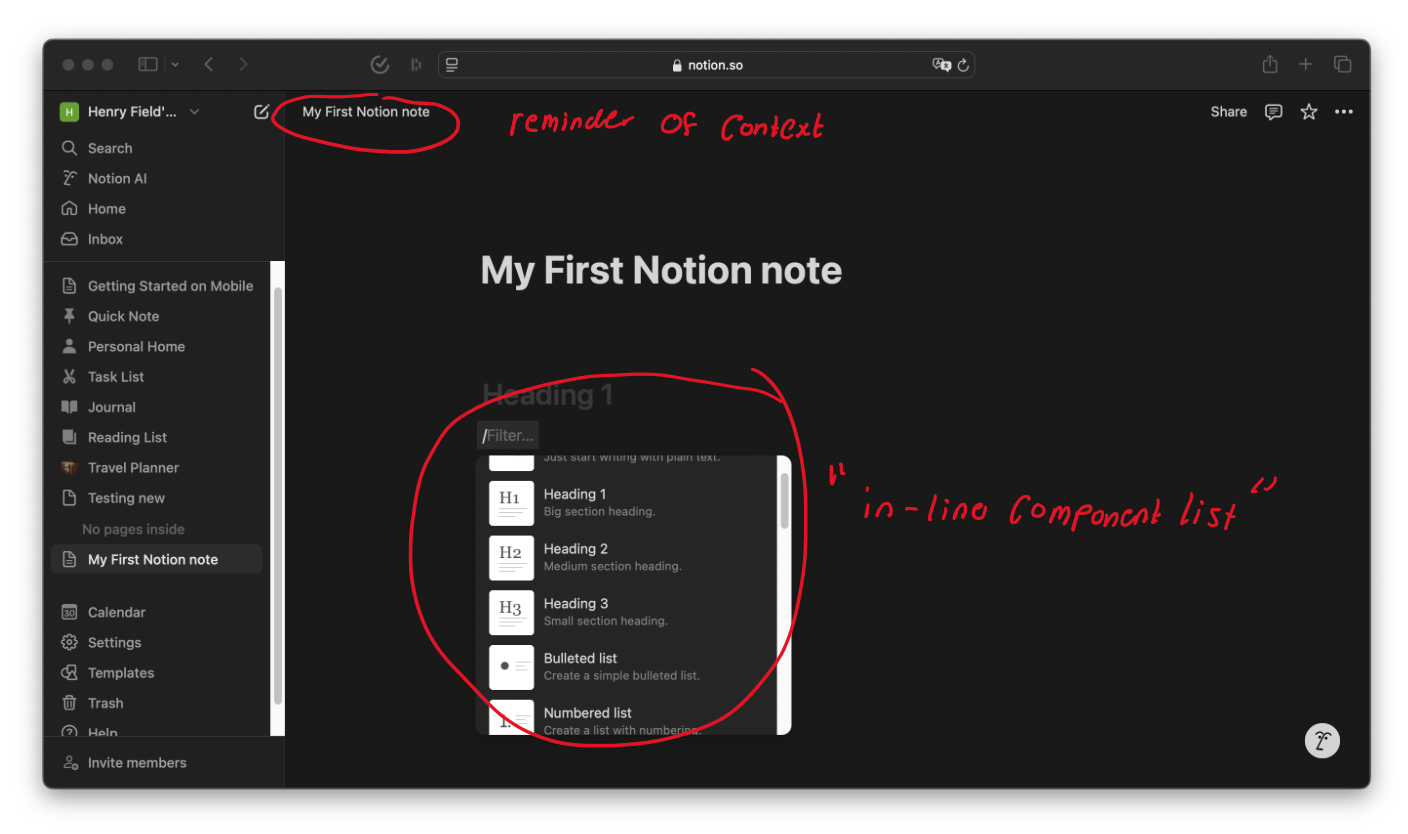
\includegraphics[width=\textwidth]{Research/15_SpecificUIResearch/media/notion4.png}
        \caption*{Notion Screenshot 4}
    \end{minipage}
    \caption{Notion UI Screenshots}
\end{figure}

Up until this point Notion had escaped my observation due to its primarily corporate focused positioning regarding pricing and advertising. Whilst this had meant it would be unfit for purpose for my target audience I still felt that was I lot I could learn from the platforms design choices and it certainly didn’t disappoint. Having explored the various features and pages of the software there is clearly a lot flexibility built into an aesthetically pleasing package. 

Within the software users are guided to create templates formed from a wide variety of components such as headings, images, bullet points etc. The method of adding these components is to type a '/' followed by the component name which brings up a floating menu, using arrow keys and enter seamlessly adds the tabs. I really like this input mechanic and whilst I've seen it used elsewhere this is by far the smoothest implementation I've used and I definitely want to incorporate this idea. While the keyboard shortcuts and navigation are powerful though the support for native handwriting input is poor and the Ui feels quite cluttered without time being spent organising it - time that I think many users wouldn’t want to spend. This makes it feel to me like a more polished form of obsidian, incredibly powerful but not designed for the average person to run with from day one.

I feel that the document editor as a whole is hugely inspirational as a content noting platform and I see my end artifact utilising a very similar system to give users the fastest typing experience. This approach does have one downside however predominantly in the lack of flexibility

\subsection*{Logseq}
\begin{figure}[H]
    \centering
    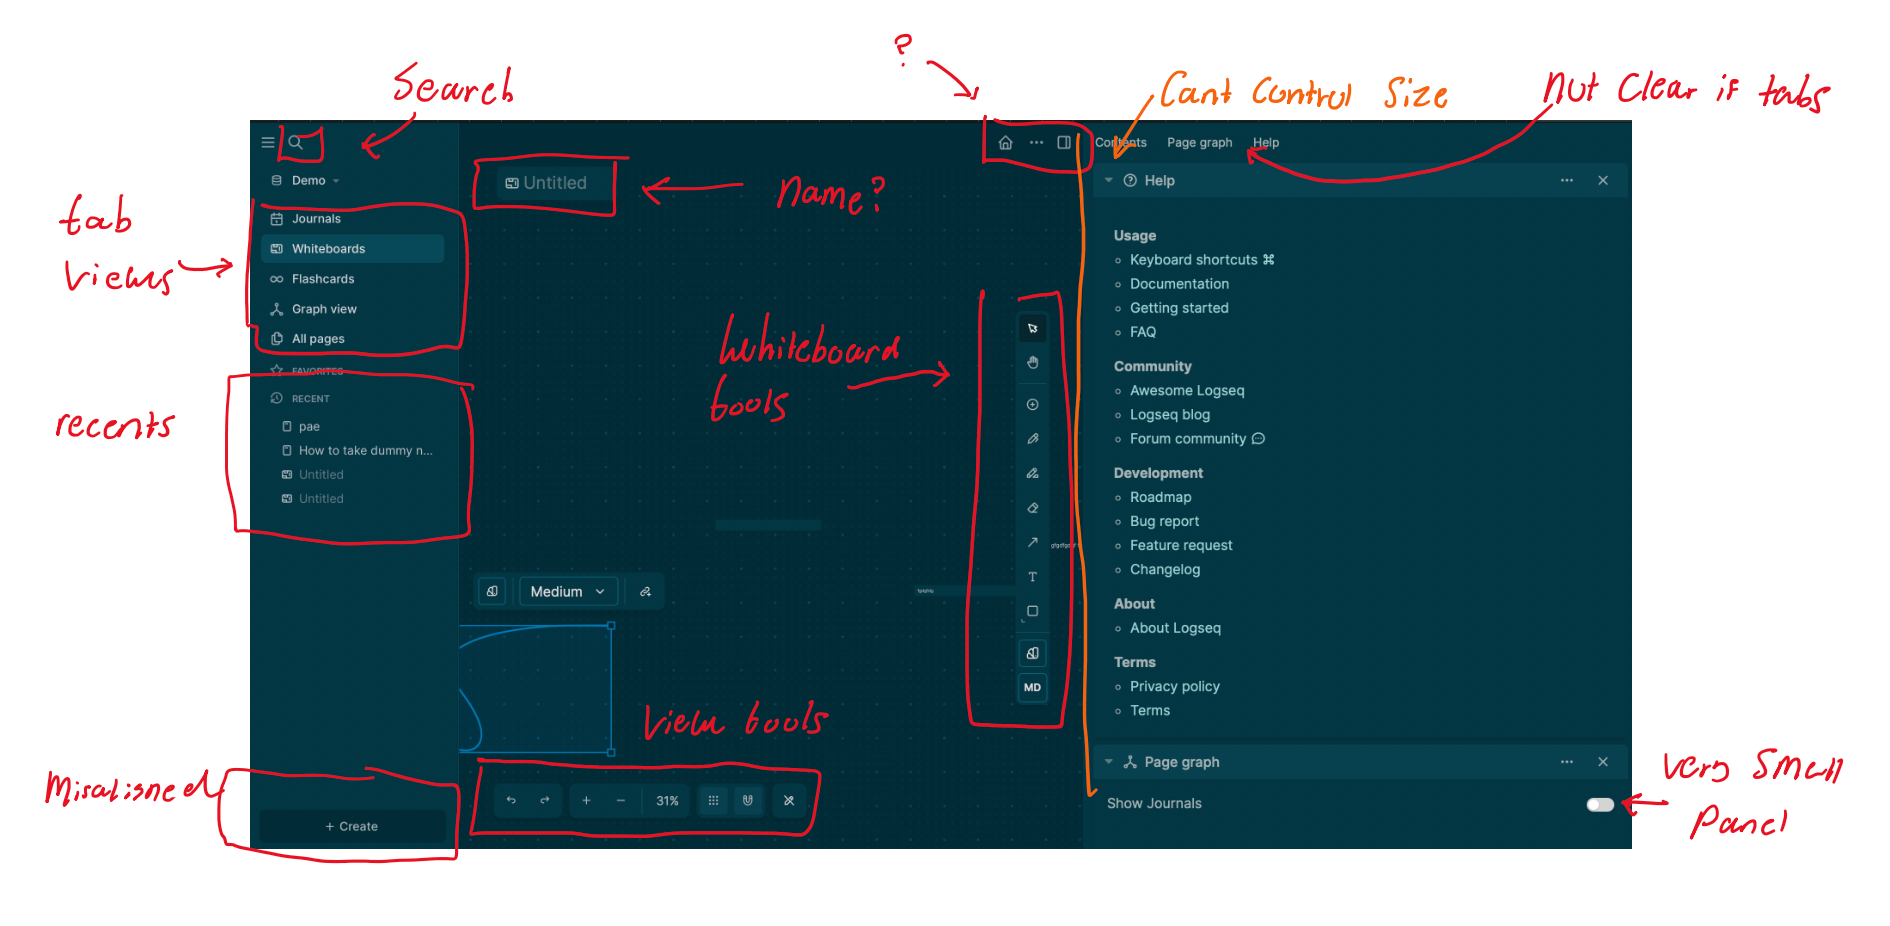
\includegraphics[width=0.8\textwidth]{Research/15_SpecificUIResearch/media/logseq.png}
\end{figure}
This is much more niche and lesser known notes application that encompasses many of the note linking feature I am building (and even a lot more), while it is undeniably powerful at finding and linking content, this does come at a cost. The user interface quickly becomes cluttered and quite confusing and even having read the manual, I was finding myself lost in menus when trying to accomplish simple tasks, this UI leaves a lot be desired. Once again though it makes use of tabs to help separate out workspaces which I do like 

Takeaways:
\begin{itemize}
    \item Nice visible recent view to switch between notes
    \item Documentation built into website (don’t have to look externally)
    \item Every popup appears by the cursor making them hard to lose
\end{itemize}
